\documentclass{article}

\usepackage{graphicx}
\usepackage{color}
\usepackage{listings}
\lstset{language=Go,
  basicstyle=\ttfamily\scriptsize,
  keywordstyle=\color{blue}\ttfamily,
  stringstyle=\color{red}\ttfamily,
  commentstyle=\color{green}\ttfamily}
\usepackage{subfiles}
\usepackage[utf8]{inputenc}

\title{Appunti su Golang - memory management}
\author{Leonardo Gonfiantini}
\date{}

\begin{document}

\maketitle

\section{La memoria in un programma}

Come sappiamo la memoria all'interno di un programma si divide principalmente in stack e heap, a seconda di come la variabile verra dichiarata risiedera in uno dei due spazi.

\begin{figure}[h!]
  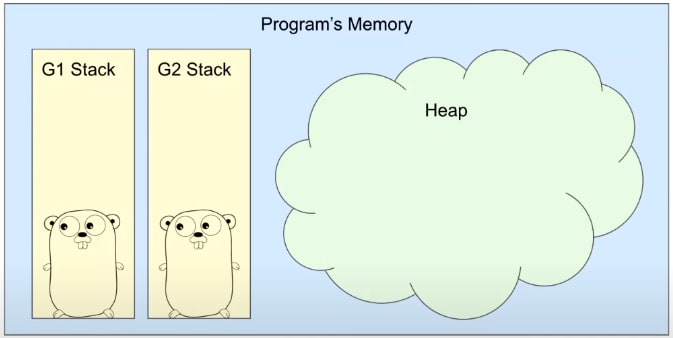
\includegraphics[width=\linewidth]{heap-stack.jpeg}
  \caption{Rappresentazione semplice della memoria}
  \label{fig: go1}
\end{figure}

L'immagine sopra rappresenta due goroutine con il loro stack separato, e l'heap del programma in generale.

\section{Come allocare memoria}
In golang la memoria viene allocata tramite l'utilizzo di due metodi:
\begin{itemize}
    \item new()
        \begin{itemize}
            \item Alloca la memoria ma non la inizializza
            \item Ritorna un indirizzo di memoria
            \item Zeroed storage
        \end{itemize}
    
    \item make()
        \begin{itemize}
            \item Alloca la memoria e la inizializza
            \item Ritorna un indirizzo di memoria
            \item non Zeroed storage
        \end{itemize}
\end{itemize}

Di solito viene utilizzato il metodo make(), la principale differrenza e' che con new() non occupiamo ancora spazio all'interno dell'heap mentre con make() occupiamo gia lo spazio.


\subfile{sections/go-manage}

\subfile{sections/go-garbage-collector}

\end{document}


